\chapter{Wide field image synthesis}
In this chapter we discuss how the Radio Interferometric Measurement Equation can be inverted to obtain a synthesized image of the radio sky. First an overview of the imaging pipeline is given, before
delving into the finer details of creating what is known as ``dirty'' images of the sky and correcting the wide field distortions introduced in the images when breaking the assumptions made when the images 
are synthesized using a Fast Fourier Transform. Finally we discuss previous literature on acceleration of the correcting process, before moving onto the design of our imager in the following chapter. Before
continuing readers not familiar should refer to Appendix~\ref{chp_DSP} for a refresher on basic signal processing concepts.
\section{The calibration, imaging and deconvolution pipeline}
The RIME can be thought of as the equation that predicts what measurement the telescope should make, given a model radio sky (\emph{intensity distribution}), telescope behavior and environmental effects as inputs. 
If all the information is known the inversion of this equation is as simple as taking an inverse Fourier Transform. To see why this is true consider that the continuous sky is simply an infinite sequence of 
shifted and scaled impulses (or delta functions), where each impulse is infinitesimally narrow, has an area of 1 and is infinitely high at the shifted position (zero everywhere else). The Fourier transform 
of each of the delta functions is simply:
\begin{equation}
 \label{eqn_delta_response}
 h(u,v) := \int_{-\infty}^\infty\int_{-\infty}^\infty \delta(l-l_\Delta,m-m_\Delta)e^{-2\pi i(ul+vm)}dldm
\end{equation}
Observe that this is practically the same as the RIME. If the delta functions are replaced with the scaled intensities over infinitesimally small areas of the sky as defined previously and the direction dependent and
independent terms are added in the convolution integral the two integrals are practically identical, apart from the $w(\sqrt{1-l^2-m^2}-1)$ term in the complex exponent and the $n = \sqrt{1-l^2-m^2}$ in the denumerator. 
For narrow fields of view these terms are negligible. We will revisit this assumption later on when discussing the wide field problem.

In order to get the \emph{observed} intensity distribution back the Fourier transform can simply be inverted. However, inversion is not all the synthesis imaging problem entails; a distinction has to be drawn
between the \emph{observed} and \emph{true} radio sky: how much of the \emph{true} radio sky can be recovered, given the imperfect measurements made with a radio interferometer over a limited amount of time? Foremost, the
effects of limited sampling in the measurement/Fourier space (uv plane) must be considered. Formally the tracks depicted in Figure~\ref{fig_evla_observation} is called the sampling function and is defined as being 1 wherever 
a measurement is made and 0 everywhere else. The observed measurements (\emph{visibilities}) are therefore a multiplication with this sampling function, $S(u,v)$:
\begin{equation}
 V_{\text{obs}}(u,v) := V_{\text{RIME}}(u,v)S(u,v)
 \label{eqn_observed_vis}
\end{equation}

When equation~\ref{eqn_observed_vis} is inverted the extent of the problem becomes apparent:
\begin{equation}
 I_{\text{obs}}(l,m) = (G_p(t,\nu)D_p(l,m,t,\nu)I_{\text{true}}(l,m)D_q^H(l,m,t,\nu)G_q^H(t,\nu))*\psf{(l,m,\nu)} + \eta
\end{equation}
where the G terms are the directional independent gains, the D terms are the directional dependent gains and the Point Spread Function, $\psf$, is the Fourier Transform of the sampling function, $S$. Since
the u,v coordinates depend on the wavelength the $\psf$ in turn also scales depending on wavelength. $\eta$ represents the background noise level that depends on system temperature, integration time and integration
bandwidth as mentioned previously.

Not all the information we need to accurately reconstruct the true intensity distribution, $I_{\text{true}}$, is available. In fact the $\psf$ alone provides a challenging
problem by itself. The more complete the sampling function, the more accurate we can reconstruct the image. If measurements are taken over too short an observation there is
no hope of deconvolving most of the $\psf$ from the image. Even more concerning is the fact that the directional dependent effects cause a time-dependent convolution with the
true measurements and serve to modulate different parts of the synthesized image at different levels during the course of an observation. Figure~\ref{fig_psf} shows how the 
$\psf$ gradually improves with longer observation time, while Figure~\ref{fig_model_convolution} provides a good illustration of the challenge astronomers face 
when just considering the effects of limited sampling on the true sky, let alone telescope sensitivity and the direction dependent and independent effects.
\begin{figure}[h]
 \begin{mdframed}
 \centering
 \begin{subfigure}[b]{0.24\textwidth}
  \includegraphics[width=\textwidth]{images/evla_observation_psf/5min.png}
  \caption{5 min snapshot}
 \end{subfigure}
 \begin{subfigure}[b]{0.24\textwidth}
  \includegraphics[width=\textwidth]{images/evla_observation_psf/30min.png}
  \caption{30 min}
 \end{subfigure}
 \begin{subfigure}[b]{0.24\textwidth}
  \includegraphics[width=\textwidth]{images/evla_observation_psf/6hr.png}
  \caption{6 hr}
 \end{subfigure}
 \begin{subfigure}[b]{0.24\textwidth}
  \includegraphics[width=\textwidth]{images/evla_observation_psf/12hr.png}
  \caption{12 hr}
 \end{subfigure}
 \caption[EVLA Point Spread Function evolution]{Here the Point Spread Function is shown for various observation lengths on the EVLA D-configuration at $\delta=30^\circ$. The PSF gradually 
 becomes more defined with longer observation time. Removing the repeating lobe-like structure around the source (clearly visible in the longer observations) is the primary goal of 
 deconvolution, since it both suppresses fainter sources and adds structure and amplification to the background noise in the image.}
  \label{fig_psf}
 \end{mdframed}
\end{figure}

\begin{figure}[ht!]
 \begin{mdframed}
 \centering
 \begin{subfigure}[b]{0.39\textwidth}
  \includegraphics[width=\textwidth]{images/evla_lena_observation/model.png}
  \caption{``True''/model sky}
 \end{subfigure}
 \begin{subfigure}[b]{0.39\textwidth}
  \includegraphics[width=\textwidth]{images/evla_lena_observation/real_FT.png}
  \caption{Real component of measurement/fourier space, shifted so that the DC component is at the centre pixel.}
 \end{subfigure}
 \begin{subfigure}[b]{0.34\textwidth}
  \includegraphics[width=\textwidth]{images/evla_lena_observation/30min.png}
  \caption{Dirty image after 30 min}
 \end{subfigure}
 \begin{subfigure}[b]{0.34\textwidth}
  \includegraphics[width=\textwidth]{images/evla_lena_observation/6hr.png}
  \caption{Dirty image after 6 hrs}
 \end{subfigure}
 \begin{subfigure}[b]{0.34\textwidth}
  \includegraphics[width=\textwidth]{images/evla_lena_observation/12hr.png}
  \caption{Dirty image after 12 hrs}
 \end{subfigure}
 \begin{subfigure}[b]{0.34\textwidth}
  \includegraphics[width=\textwidth]{images/evla_lena_observation/24hr.png}
  \caption{Dirty image after 24 hrs}
 \end{subfigure}
 \caption[Effect of observation time on dirty image synthesis]{If the model sky looked like the standard Lenna image then limited sampling with an interferometer will produce a ``dirty'' image that
 must be devonvolved in order to recover as much of the ``true''/model sky as possible.}
  \label{fig_model_convolution}
 \end{mdframed}
\end{figure}

Referring back to the sampling tracks in Figure~\ref{fig_evla_observation} highlights a further (but minor) complication with the PSF: there are clearly more short baselines than long baselines. The resulting effect on this non-uniform
weighting in the sampling function is a broadening of the $\psf$ and by implication an bias towards resolving extended structure in the image space. In order to resolve finer (compact) emission structure in the image
it is necessary to divide through by the number of samples in the neighborhood of each point in the measurement space, in order to \emph{uniformly} weight the synthesized image. This highlights an important aspect about
interferometers in general: the $\psf$ acts very similar to a high-pass filter. Adding longer baselines to an array increases the compactness of the $\psf$, which in turn serves to resolve higher frequency structure (edges, points, etc.)
in the image. This is not always desirable - observing extended emission sources is equally important, which requires only short baselines and more robust weighting methods are possible.

Along with the weighting by a density function the measured visibilties are also tapered by a Gaussian-like function in order to control the shape of the $\psf$ and
drive down the first few sidelobes of the $\psf$ at the slight expense of broadening its main lobe. The final weight also contains the inverse of the expected 
(constant if calibration is successful) variance of the measurement in order to improve the signal to noise level in the synthesized image. The technicalities are
not very important in our discussion, but the reader may refer to Briggs et al. \cite[Lecture 7]{taylor1999synthesis} and \cite[p. 387-399]{thompson2008interferometry} for 
more details.

This brings us to consider a strategy to deconvolve the extended lobe structure of the $\psf$ from the images. In order to achieve this goal we make an assumption about the distribution of sources in the sky, in that the radio
sky is mostly void of emission. If we further assume most sources are compact point-like sources it gives us one possible strategy to remove some of the $\psf$ structure as stated in CLEAN, Algorithm~\ref{alg_clean}.
\begin{algorithm}
  \begin{algorithmic}
  \STATE {Given a dirty image, $d$ of size $n \times m$ pixels}
  \STATE {Given a synthesized $\psf$ of size $2n \times 2m$}
  \STATE {Let $c$ be an all-zero cleaned image of size $n \times m$}
  \STATE {Given the loop gain $0.0 \leq \gamma \leq 1.0$}
  \STATE {Let $R_p = \infty$}
  \STATE {Let $R_c = \infty$}
  \REPEAT
      \STATE {Let $b$ be the position of the maximum value in $d$}
      \STATE {Set $c[b] = c[b] + \gamma\max{d}$}
      \STATE {Subtract from $d$ the scaled beam $\gamma\max{d}\psf$, centred on position $b$}    
      \STATE {Set $R_p = R_c$}
      \STATE {Set $R_c = \frac{\max{d}}{\rms{d}}$}
  \UNTIL {$|R_p - R_c| \leq \epsilon$ \OR maximum iterations reached} 
  \STATE {Convolve $c$ with gausian-like function with half-amplitude width equal to that in the \psf}
  \STATE {Set $c[...] = c[...] + d[...]$, ie. add the residual noise back into the cleaned image}
  \end{algorithmic}
  \caption{The H\"ogbom CLEAN algorithm}
  \label{alg_clean}
\end{algorithm}

Although CLEAN was initially intended only to work on a sky consisting of point sources, practice shows that it
deconvolves regions of extended emission as well. The output is then a collection of clean components spaced closely
together. 

The $\psf$ subtraction in the image / sky domain for every detected source is a relatively expensive operation. One of the
most notable adaptions to CLEAN is the Cotton-Schwab major-minor cycle adaption to the algorithm. Here only a truncated
$\psf$ (up to the first few sidelobes) is subtracted in the image domain. The resulting clean model is then converted back
to the continuous measurement domain (here again the measurement is predicted by the RIME) and then subtracted from the 
observed visibilities. In fact this major-minor cycle approach works well when deconvolving multiple adjacent fields. 

The convergence criteria of the algorithm is well beyond the introductory discussion here. Refer to Thompson et 
al. \cite[ch 11]{thompson2008interferometry} for a more detailed discussion and further reading on the topic. More
recently new sparse synthesis and analysis approaches has been suggested as alternatives to CLEAN. An example is the 
MORESANE \cite{dabbech2015moresane} algorithm.

In addition to the $\psf$ deconvolution problem is the telescope calibration problem. Apart from removing unwanted
radio interference and erroneous measurements through flagging and solving for varying instrumental gains, it is also
necessary to calibrate known, and solve for unknown directional-dependent effects. One of the more pronounced directional-dependent 
effects is the antenna primary beam and its associated polarization effects in wide-field imaging. We will return
to ways of solving this problem after discussing the projection effect introduced by the $w(n-1)$ term in the RIME.

To summarize this discussion the general imaging pipeline is illustrated in Figure~\ref{fig_img_pipeline}. Next we will discuss
how images can be efficiently synthesized (Fourier-inverted / ``backwards-processed'') using a narrow-field approximation.
\begin{figure}[h]
 \begin{mdframed}
 \centering
 \begin{tikzpicture}[node distance=4.5cm]
  \node (start) [start] {};
  \node (dical) [process, right of=start] {Direction independent calibration \& flagging};
  \node (backward) [process, right of=dical] {Fourier inversion (synthesis/``backward computation'')};
  \node (minor) [process, below of=backward] {Minor cycle model estimation};
  \node (prediction) [process, below of=minor] {Continuous measurement/visibility calculation (``Prediction'') using the RIME};
  \node (major) [process, left of=prediction] {Major cycle residual calculation};
  \node (converged) [decision, above of=major] {Converged};
  \node (finalize) [process, left of=converged] {Clean map creation};
  \node (stop) [stop, below of=finalize] {};
  \draw [rarrow] (start) -- node [yshift=0.3cm] {Observed} (dical);
  \draw [rarrow] (dical) -- (backward);
  \draw [rarrow] (backward) -- node [anchor=west] {``Dirty''} (minor);
  \draw [rarrow] (minor) -- node [anchor=west] {``Model''} (prediction);
  \draw [rarrow] (prediction) -- node [yshift=0.3cm] {$V(u,v)$} (major);
  \draw [rarrow] (major) -- (converged);
  \draw [rarrow] (converged) -- node[yshift=0.3 cm] {yes} (finalize);
  \draw [rarrow] (converged) -- node[anchor=west] {no} (backward);
  \draw [rarrow] (finalize) -- (stop);
 \end{tikzpicture}
 \caption[Imaging pipeline]{Here the traditional imaging pipeline is shown. The known directional-dependent calibration terms are taken 
 into account during the ``backwards'' inversion step, while the unknown slowly varying directional-dependent effects can be solved for
 if enough about the model sky is known.}
 \label{fig_img_pipeline}
 \end{mdframed}
\end{figure}

\section{Narrow field synthesis using the FFT}
 There are generally two techniques used to approximate the fourier transforms between the observed visibilities and the (dirty) image. Either a brute force Direct Fourier Transform is taken where each grid point is approximated through a brute-force
 evaluation over all the observed visibilities (M of them in total). This approach requires on the order of $N^2M \approx N^4$ sine and cosine evaluations (where N is the size of a single dimension of a square grid) for a large number of visibilities. 
 The direct inversion algorithm boils down to a M summations of complex multiplications over the entire image \cite[Lecture 7]{taylor1999synthesis}. This equation can be amended to be as accurate as needed, taking per-pixel effects into 
 account if necessary:
 \begin{equation}
  (\forall c\in\text{correlations})(\forall\text{ pixels }l,m) I_{\text{observed},c}[l,m] = \frac{1}{M}\sum_{k=1}^{M}{\frac{V_{c,\text{observed}}}{n}[u,v]e^{2\pi i (ul + vm + w(n-1))}}
 \end{equation} 
 
 The first approach is prohibitively expensive when the number of baselines grows or the observation time increases, considering that the operation will be called upon multiple times in a major-minor deconvolution cycle. Instead astronomers rely
 on a simple \emph{planar} approximation. This second approach employs the Fast Fourier Transform (see Cochran et al. \cite{cochran1967fast} for algorithmic details). Instead of having complexity order $N^4$ the two dimensional Fast Fourier 
 Transform can be computed with roughly $2N^2\log{N}$ steps. There are three very serious problems to consider though:
 \begin{enumerate}
  \item The Fast Fourier Transform yields a \emph{tangent planar approximation} to the sky dome: the synthesized image is only accurate near the phase centre (by convention the center pixel) of the image.
        This implies that the FFT may only be used when $\sqrt{1-l^2-m^2} - 1 \ll 1$. When doing wide field synthesis this assumption is broken and have to be corrected for.
  \item The Fast Fourier Transform only operates on \emph{regularly sampled} data. This statement simply means that the data has to be sampled on a uniformly spaced grid in order to 
	apply the two dimensional FFT. This resampling step (essentially a variant of image upsampling) is very computationally expensive: as we will see it quickly comes to 
	dominate the entire synthesis process. On the other end of the pipeline the prediction step suffers from the same affliction: a FFT can again be employed when going 
	from the model sky to continuous measurements, but then the regularly spaced samples have to be resampled to continuous coordinates.
  \item The regularly sampled FFT assumes the signal (in this context the signal is the sky) is periodic (in other words it repeats: sources outside the field of view of the produced image is flipped back into the image on the opposite side. This 
	introduces the necessity to filter the image with a filter that only passes signal that is in the field of view being considered and stops any energy 
	outside the field of view.
 \end{enumerate}
 The second and third problems are related and for now our discussion will be focused on providing a solution to address them. The first problem will be discussed in
 the next section.
 
 We will use the terms ``interpolation'' and ``resampling'' interchangeably throughout this thesis. By these terms we refer to a process that 
 either takes a set of continuous samples as input and yields a discretized set of samples as output (``gridding'') or working in the opposite 
 direction (appropriately referred to as ``degridding''). There is no single best way to interpolate data onto a regularly spaced grid 
 and it necessary to consider multiple strategies to complete this task. The resampling problem is shared between the many fields including, 
 but not necessarily limited to, the astronomical and medical imaging subfields, and as such literature from both fields can be considered in 
 the discussion. An excellent comparative discussion on image interpolation is given by Th\'evenaz et al. \cite{thevenaz2000image}, while
 Thompson and Bracewell \cite{thompson1974interpolation} gives a detailed overview and comparison of different interpolation techniques when it comes to 
 resampling the visibility measurements produced by an interferometer. Briggs et al. \cite[Lecture 7]{taylor1999synthesis} and 
 Thompson et al. \cite[p. 387-399]{thompson2008interferometry} give concise discussions of the technical considerations that must be taken into 
 account in the synthesis step. Our discussion highlights some key considerations and findings from these works.
 
 Thompson and Bracewell \cite{thompson1974interpolation} suggests a radial interpolation strategy, but it assumes
 that the baseline tracks (as depicted earlier) are concentric circles of an East-West array (at high declinations for instance). Instead a 
 more non-exact interpolation-by-convolution strategy is widely followed here. In radio astronomy the resampling step focuses on a 
 variant of the relatively fast class of linear interpolation operations:
 \begin{equation}
   \label{eqn_interp_op}
   (\forall f(a)\in\mathbb{C},\phi(b)\in\mathbb{C})f(x) = \sum_{k\in Q\subseteq\mathbb{R}^2}{f(k)\phi(x-k)}
 \end{equation}
 The constant-selection function $\phi$ can be one of the myriad of functions proposed in the literature. These include linear, Lagrange, sinc, 
 Gaussian, modified B-spline, etc. and may additionally be windowed by one of the large number of window functions as in the case of the sinc function, 
 for example Hamming, Hanning, Blackman, Kaiser-Bessel, along with many others.
 
 Notice that if the resampling was to be done on data that was already discretely sampled (traditional upsampling) and the constant 
 selection function $\phi$ was evaluated at the resulting integer positions, Equation~\ref{eqn_interp_op} would be a discrete convolution as it is
 normally defined. Instead the operator as it stands here is not the regular convolution sum and should be thought of as an approximate convolution. 
 Strictly speaking convolutional gridding and degridding are not exact interpolation operations as Thompson et al. \cite{thompson2008interferometry} and 
 Sze Tan \cite{tan1986aperture} points out, but rather interpolation-like (or as Briggs et al. \cite[Lecture 7]{taylor1999synthesis} puts 
 it: a \emph{non-discrete integral convolution approximation}).
 
 It is useful to think of this \emph{non-discrete integral convolution} operator in terms of the ordinary upsampling operation. As with upsampling (where
 the data is already discretized) the space in-between samples are filled with zero value\footnote{``Zero-stuffed'' in DSP nomenclature}, only here the zeros
 are added in-between continuous samples at integral spacings. Just as with ordinary upsampling it is then necessary to ``smoothen'' the new data points 
 between the measured points using some form of interpolation / convolution, in order not to introduce new high frequency terms (sudden jumps) in the 
 higher resolution image. It is quite important to realize however that in the gridding the data is simply smeared out into the continuous
 measurement space and by implication also over the newly inserted zeros. The rationale behind degridding can be explained using a very similar downsampling 
 argument. To help visualize this ``convolutional gridding'' process refer to Figure~\ref{fig_gridding}.
 \begin{figure}[h]
  \begin{mdframed}
   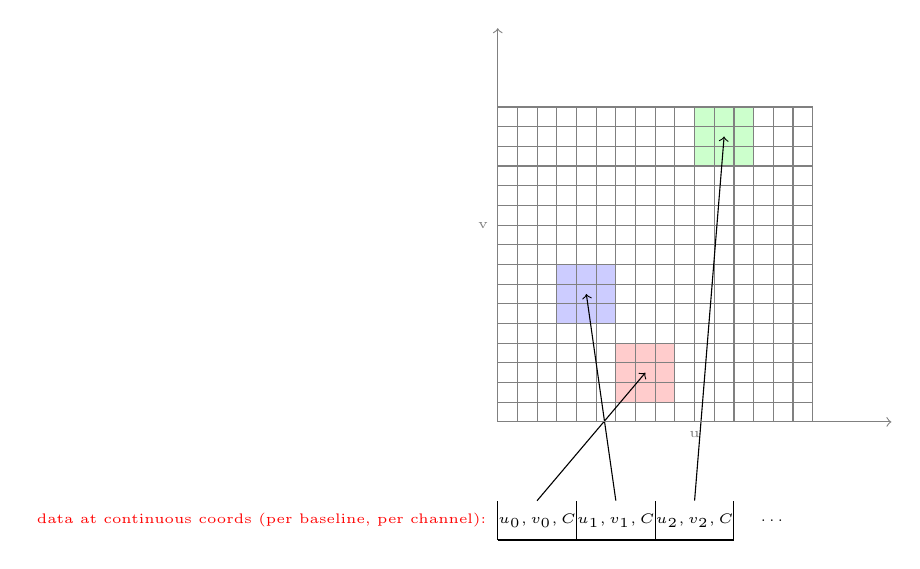
\begin{tikzpicture}[font=\tiny]
    \filldraw[fill=red!20] (4.50,1.75) rectangle (5.25,2.5);
    \filldraw[fill=blue!20] (3.75,2.75) rectangle (4.50,3.50);
    \filldraw[fill=green!20] (5.50,4.75) rectangle (6.25,5.5);
    \draw[step=0.25,gray,thin] (3,1.5) grid (7,5.5);
    \draw[red] node at (0,0.25) {data at continuous coords (per baseline, per channel):};
    \draw node at (6.5,0.25) {\dots};
    \draw[step=1,black] (3,0) grid (6,0.5);
    \draw node at (3.5,0.25) {$u_0,v_0,\mathbb{C}$};
    \draw node at (4.5,0.25) {$u_1,v_1,\mathbb{C}$};
    \draw node at (5.5,0.25) {$u_2,v_2,\mathbb{C}$};
    \draw[->] (3.5,0.5) -- (5-0.125,2.25-0.125);
    \draw[->] (4.5,0.5) -- (4.25-0.125,3.25-0.125);
    \draw[->] (5.5,0.5) -- (6-0.125,5.25-0.125);
    \draw[->,gray] (3,1.5) -- (8,1.5) node[below,pos=0.5]{u};
    \draw[->,gray] (3,1.5) -- (3,6.5) node[left,pos=0.5]{v};
   \end{tikzpicture}
   \caption[Illustration of convolutional gridding]{Each observed visibility (per channel and baseline) is centered at some precomputed coordinate in continuous u,v space and 
    is ``convolved'' with some function C, which extends only to finite ``full support'' region as illustrated. The result is binned in a regularly spaced grid. 
    This process essentially spreads each visibility out over a larger area in u,v space. It should be clear that this is not the standard convolution 
    operator as defined in Appendix~\ref{chp_DSP}. After all the observed visibilities have been gridded an Inverse Fast Fourier Transform is performed 
    and a correcting function is applied. Each correlation term (or Stokes sum) is typically resampled and transformed to its own image.}
   \label{fig_gridding}
  \end{mdframed}
 \end{figure}
 
 The interpolated measurements taken at the grid points are not known exactly, and normally in interpolation techniques it is 
 hoped that the variance of this error is small as soon as the step size in the resampling process becomes infinitesimally narrow. 
 In the context of radio astronomy the ``significantly oversampled'' criterion is not normally met because of the significant amounts 
 of memory this will require, especially considering the sizes of the arrays currently under construction. Instead, only a 
 \emph{critically sampled} image is usually produced during synthesis. Importantly note that ``critically sampled'' refers to 
 the Shannon-Nyquest sampling criterion:
 \begin{equation}
  \label{eqn_img_sampling}
  \begin{split}
    \Delta{l} &= \frac{1}{2N_l\Delta{u}}\text{, }\Delta{l}:=\frac{1}{l_{\text{max}}},\Delta{u}:=\frac{1}{u_{\text{max}}}\\
    \Delta{m} &= \frac{1}{2N_m\Delta{v}}\text{, }\Delta{m}:=\frac{1}{m_{\text{max}}},\Delta{v}:=\frac{1}{v_{\text{max}}}\\
  \end{split}
 \end{equation}
 Here $\Delta{l}$ and $\Delta{m}$ are the pixel sizes given in degrees (or equivalently arcminutes, arcseconds or radians). If the images are sampled are 
 subsampled (change the equality to $>$) the longest baselines will fall off the uv grid and angular resolution will be lost. 
 
 This sampling criterion alone justifies our statement that the Fourier response of the resampling function should be considered of higher priority
 than the approximation criterion, unlike in other contexts where interpolation quality may be the most important. The energy reduction properties of
 $\phi$ can be stated in terms of maximizing the following integral ratio for all square-integrable $\phi$ functions\footnote{It is possible to
 define another criterion here, for example to promote accurate interpolation over energy concentration. Sze Tan \cite{tan1986aperture} for 
 instance defined this as minimizing the difference between the Direct Transform and the FFT approach}:
 \begin{equation}
  \label{eqn_aliasing_energy}
  \frac{\int_{\text{FOV}}{|[\mathcal{F}\phi](l,m)|^2dS}}{\int_{-\infty}^{\infty}{|[\mathcal{F}\phi](l,m)|^2dS}}
 \end{equation}
 
 To better understand why these repeating or ``aliased sources'' occur in the first place we have to define the gridding operation somewhat more 
 rigorously. Each (discrete) measurement taken by an interferometer in the continuous uv space  is ``convolved'' with a two-dimensional interpolation 
 function in order to create a continuous function. This function is then discretized again onto a set of regular coordinates by a 
 ``bed-of-nails'' function. Mathematically we can say:
 \begin{equation}
  V_{\text{gridded}}[u,v] = [V_{\text{sampled,observed}}(u,v)*\phi(u,v)]\frac{\III(u,v)}{\Delta{u}\Delta{v}}
 \end{equation}
 where $\III$ is the shah function defined as:
 \begin{equation}
  \III(u/\Delta{u},v/\Delta{v})=\Delta{u}\Delta{v}\sum_{j=-\infty,j\in\mathbb{Z}}^{\infty}{\sum_{i=-\infty,i\in\mathbb{Z}}^{\infty}{\delta{(u-j\Delta{u},v-i\Delta{v})}}}
 \end{equation}
 
 Convolution with the Fourier transform of the shah function (composed itself by many band-limited impulses) creates a sum of periodic functions
 in the image domain \footnote{It is useful to note that the Fourier transform of a band-limited (non-zero over a finite range) function 
 such as a box function is a function that stretches over an infinite support region}. The result is a periodic field of view that repeats at
 $M\Delta{l}$ and $N\Delta{m}$ for an $M\times N$ image (ie. at multiples of the field of view). In practice not all the energy from 
 these replicated fields can be stopped at the edge of the field of view, and this is responsible for the aliasing seen in the images. Further
 truncation of the shah function to represent only a single field of view, as well as the truncation of the convolving function also 
 contribute to the aliasing. It should be understood that the $\psf$ sidelobes from sources outside the field of view that fall legitimately inside
 the field of view are not removed and this will raise the noise levels inside a deconvolved image if the sources responsible for those sidelobes are not
 included in the deconvolved model.
 
 The $\phi$ functions considered here all have the property of \emph{separability}. By this it is implied that $\phi(u,v) = \phi(u)\phi(v)$. We will return
 to a discussion of this later on when discussing w-projection. For now the discussion will focus on functions of one variable.
 
 After aliasing speed becomes a major consideration. Due to the large measurement datasets produced with larger arrays the convolutional resampling process
 has to be fast; the complexity of the resampling step grows as $MC^2$, where C is the support size of the convolution filter. Therefore
 the convolution function $\phi$ is normally pretabulated for a given support size in grid steps. Additionally it is very important to oversample
 the precomputed $\phi_{\text{filter}}$ to reduce conserve the spatial relation in the measured coherence function and to 
 attain \emph{high dynamic range images} (peak value to noise level in the image).
 
 To further understand why the filter has to be significantly oversampled (usually dozens of times) consider that interferometers take measurements 
 in the Fourier space, where any rounding operation (or snapping) of the u,v coordinates in either the grid
 or the filter will cause fringe-like decorrelation in the observed sources. Th\'evenaz et al. \cite{thevenaz2000image} also
 points out that $\phi$ must be symmetrical (ie. $\phi{(x)} = \phi{(-x)}$ and $\phi_{\text{filter}}[x] = \phi_{\text{filter}}[-x]$) to preserve 
 the image phase correctly.

 The image phase consideration effectively precludes using nearest-neighbor\footnote{or \textit{cell-summing} techniques as 
 Thompson and Bracewell \cite{thompson1974interpolation} puts it} interpolation. The nearest neighbour technique simply snaps (box function) 
 points close to the grid point into the sum at that point, without any consideration on the visibility's distance from the grid point. Additionally 
 the Fourier transform of the box function is an \emph{infinite} $\sinc$ function.  Due to the fact that the $\sinc$ function slowly ripples out 
 toward $\infty$ it is not a good response when it comes to reducing the unwanted energy from sources that fall outside the field of view.
 
 What makes convolutional gridding a more attractive approach to cell-summing is the fact that the distance between the grid point and the
 measured uv point is taken into consideration when picking a set of convolution weights from the oversampled filter shown in 
 Figure~\ref{fig_filter}. The fractional offset is simply calculated between the nearest regular grid coordinate and measured uv coordinate and is used to pick
 the nearest filter value in the oversampled filter.
 
 \begin{figure}[h]
  \begin{mdframed}
   \centering
   \begin{tikzpicture}[font=\tiny]
    \draw node at ({0*3},0.5) {$\lvert$};
    \draw node at ({0.2*3},0.5) {*};
    \draw node at ({0.4*3},0.5) {*};
    \draw node at ({0.6*3},0.5) {*};
    \draw node at ({0.8*3},0.5) {*};
    \draw node at ({1*3},0.5) {$\lvert$};
    \draw node at ({1.2*3},0.5) {*};
    \draw node at ({1.4*3},0.5) {*};
    \draw node at ({1.6*3},0.5) {*};
    \draw node at ({1.8*3},0.5) {*};
    \draw node at ({2*3},0.5) {$\lvert$};
    \draw node at ({2.2*3},0.5) {*};
    \draw node at ({2.4*3},0.5) {*};
    \draw node at ({2.6*3},0.5) {*};
    \draw node at ({2.8*3},0.5) {*};
    \draw node at ({3*3},0.5) {$\lvert$};
    \draw node at ({3.2*3},0.5) {*};
    \draw node at ({3.4*3},0.5) {*};
    \draw node at ({3.6*3},0.5) {*};
    \draw node at ({3.8*3},0.5) {*};
    \draw node at ({4*3},0.5) {$\lvert$};
    
    \draw node at ({0*3},0) {1};
    \draw node at ({0.2*3},0) {2};
    \draw node at ({0.4*3},0) {3};
    \draw node at ({0.6*3},0) {4};
    \draw node at ({0.8*3},0) {5};
    \draw node at ({1*3},0) {6};
    \draw node at ({1.2*3},0) {7};
    \draw node at ({1.4*3},0) {8};
    \draw node at ({1.6*3},0) {9};
    \draw node at ({1.8*3},0) {10};
    \draw node at ({2*3},0) {11};
    \draw node at ({2.2*3},0) {12};
    \draw node at ({2.4*3},0) {13};
    \draw node at ({2.6*3},0) {14};
    \draw node at ({2.8*3},0) {15};
    \draw node at ({3*3},0) {16};
    \draw node at ({3.2*3},0) {17};
    \draw node at ({3.4*3},0) {18};
    \draw node at ({3.6*3},0) {19};
    \draw node at ({3.8*3},0) {20};
    \draw node at ({4*3},0) {21};
   \end{tikzpicture}
   \caption[Oversampled filter]{Accross the literature the definition for ``filter support or window width'' varies considerably. To illustrate the use of the
   terminology in our work a ficticious filter is shown here. Here the padded and oversampled $\phi_{\text{filter}}[x]$ is illustrated for a 3-cell full-support 
   region (half support of 1 to both sides of the centre value), padded with one value on both sides. The filter is 5x oversampled, as indicated by the asterisks
   between the bars, which represent the cell-spacing ($\Delta{u}$) used for the grid. If the measured uv coordinate falls exactly on the nearest grid 
   cell then values 6,11 and 16 are selected as interpolation coefficients. If $\round{(\fracof{(u,v)}m_{\text{oversample factor}})} = 2$ for instance 
   then 8, 13 and 18 are selected for the 3 grid points being ``convolved'' or ``smeared'' onto. In other words we place a denser bed of nails over the bed of 
   nails of the grid and select the closest set of coefficients for the convolution. Briggs et al. \cite[Lecture 7]{taylor1999synthesis} notes that this discretization
   of $\phi$ will cause a minor replication effect with a very long period of $\frac{m_{\text{oversample factor}}}{\Delta{u}}$ and 
   $\frac{m_{\text{oversample factor}}}{\Delta{v}}$ in the respective u,v directions.}
   \label{fig_filter}
  \end{mdframed}
 \end{figure}
 
 If the last observation about box functions are inverted then we arrive at a partial solution to the problem of selecting a filtering function
 that better limits aliasing energy; convolving with the \emph{infinite} $\sinc$ yields a box response in the image domain. Unfortunately it is 
 impossible to convolve with a infinite function to exactly reconstruct the sought-after box response in the image domain. It is also computationally
 prohibitive to increase the support range of the convolution filter, but without large support sizes the filter's Fourier response does not taper (or 
 ``roll off'') immediately. See Figure~\ref{fig_aliasing_nn_vs_sinc} for a comparative example of the significant difference between nearest neighbor 
 interpolation compared to even just the ordinary $\sinc$ function.
 \begin{figure}[h]
  \begin{mdframed}
    \centering
    \begin{subfigure}[b]{0.35\textwidth}
      \includegraphics[width=\textwidth]{images/ratt_aa_kernel_demo_nn.png}
      \caption{Nearest neighbor interpolation}
    \end{subfigure}
    \begin{subfigure}[b]{0.35\textwidth}
      \includegraphics[width=\textwidth]{images/ratt_aa_kernel_demo_larger_support.png}
      \caption{$\sinc$ 8x8 full support}
    \end{subfigure}
    \caption[Alias reduction]{Here a ``grid'' sky model was simulated using MeqTrees\cite{noordam2010meqtrees} and imaged with our imager, first 
    using Nearest Neighbour and then using an ordinary unwindowed $\sinc$ function. Sources that fall slightly outside the field of view are 
    aliased back in when the energy outside the field of view is not limited as expected.}
    \label{fig_aliasing_nn_vs_sinc}
  \end{mdframed}
 \end{figure}
 
 To address this problem the literature is filled with alternative windowing functions to the truncation window, of which 
 the Kaiser-Bessel window proposed by Jackson et al. \cite{jackson1991selection} yields very good results. 
 Offringa et al. \cite{offringa2014wsclean}\footnote{Special thanks goes to Andr\'e Offringa for sending me a snipped of code
 where he implemented this filtering and useful discussions around this topic} used this filter in their implementation of a 
 w-stacking (explained later) imager to great success. The Keiser-Bessel window is defined as:
 \begin{equation}
  \frac{1}{W}I_0(\beta\sqrt{1-(2x/W)^2})
 \end{equation}
 Where W is the full support of the convolution filter. See Jackson et al.\cite{jackson1991selection} for tabulated constants used 
 for $\beta$.

 An alternative to using a windowed $\sinc$ function is to use a prolate spheriodal function. These are also widely employed in 
 astronomical imagers. The Spheriodal functions have the property we're looking for, in that most of their energy is concentrated 
 over the central part of the function, as a weighted variant of Equation~\ref{eqn_aliasing_energy} as proven generally by 
 Donald Rhodes \cite{rhodes1970spheroidal}. A later analysis by Frederic Schwab \cite{schwab1984optimal} confirms the good 
 performance of the spheriodal functions in practice as anti-aliasing filters. Here the prolate spheriodal is defined as 
 for the special case that $\alpha=0$:
 \begin{equation}
  |1-(2x/W)^2|^\alpha\psi_{\alpha0}(0.5\pi W,2x/W)
 \end{equation}
 
 Here $W$ is again the full support of the the convolution filter and $x$ increases in steps of $\Delta{u}$. When $\alpha>0$ a 
 weighted energy concentration ratio is maximized instead. The $\psi_{xy}$ function is the one defined by Donald Rhodes \cite{rhodes1970spheroidal}.
 Its definition alone is well beyond the scope of this discussion, and in fact it is quite difficult to compute for arbitrary support and
 oversampling parameters.
 
 After taking the Fourier transform the tapering effects of $\phi$ may optionally be corrected for by point-wise dividing through by the Fourier transform of
 $\phi$. This does not completely eliminate $\phi$ from the resulting expression, but has the effect of flattening the response of the pass band (removes the
 tapering towards the edges of the image, but at the same time increasing the amplitudes of the aliasing-sidelobe responses.
 
 Measuring energy outside the grid-corrected image, Jackson et al.\cite{jackson1991selection} shows that the Keiser-Bessel-windowed $\sinc$ achieves 
 very similar performance to the Gaussian and Prolate Spheriodal Function for small (preferable) support regions and similar performance to the 
 prolate spheriodal for larger windows, whilst being considerably easier to compute than the latter. One possible downside to windowed sinc functions
 are their inability to reproduce a constant function as Th\'evenaz et al. \cite{thevenaz2000image} points out. A synthesized image with a non-zero 
 mean will appear either too light or too dark when compared to a model image. It is unclear if the prolate spheriodal function suffers from the same
 problem. Th\'evenaz et al. also points out that the sinc introduces blockiness in the image.
 
 Lastly it is necessary add (though this is unrelated to the discussions above) that both the Direct Fourier Transform and Fast Fourier Transform approaches
 have to scale the field of view of the image according to the cell size and number of pixels in the image. In the Fast Fourier Transform approach this is 
 achieved by scaling the measurement domain's u,v coordinates (measured in $\text{cycles}\text{m}^{-1}\text{rad}^{-1}$) such that when inverted the image
 has the desired field of view. To achieve this we use the \emph{similarity} property of the FFT:
 \begin{equation}
  \alpha^{-n}F(x/\alpha) \rightleftharpoons f(\alpha x)
 \end{equation}
 Here $n$ depends on the dimensionality of the Fourier transform. If the desired field of view (measured in radians) is multiplied to each sampled
 u,v coordinate such that the desired $-0.5\Delta{l}N_l\leq x\leq0.5\Delta{l}N_l$ field of view is satisfied in the synthesized image. It is further 
 important to note that, by convention, the gridded visibilities are shifted before Fourier transform such that the 0 frequency component 
 (``DC'' component) is at the centre of the grid and the corresponding centre of the observed field on the image is in the centre pixel of the image.
 
 To summarize the convolutional gridding process is shown in Figure~\ref{fig_synth_pipeline}.
 \begin{figure}[h]
  \begin{mdframed}
    \centering
    \includegraphics[width=0.35\textwidth]{images/convolutional_gridding_flow.png}
    \caption[Synthesis using convolutional gridding]{Here the classic synthesis by convolutional gridding and Inverse Fast Fourier transform is shown.
    The signal (u,v domain) is multiplied by a sampling function (and optionally weighted by the computed and tapered density function). Then it is convolved
    and resampled onto the regular grid, Fourier transformed and optionally grid-corrected by point wise division. Courtesy of Jackson et al.\cite{jackson1991selection}}
    \label{fig_synth_pipeline}
  \end{mdframed}
 \end{figure}
 
\section{Widefield distortions and the problem of non-coplanar baselines}
Evaluating a direct 3D analytical solution over an image cube with n layers soon becomes intractable for large images, specifically in terms of sheer memory requirements for storing these layers. Over a three dimensional cube, M (the number of visibilities),
will be reasonably sparcely sampled, and the number of complex multiplications needed per visibility is estimated to be $\frac{4\lambda B_{max}^3}{D^4}$ \cite{yashar2009tdp}. However, the approach remains embarisingly parallel and can
be scalled over multiple multicore accelerators. A detailed comparison between the throughput achievable by using an analytical approach, compared to convolutional gridding approaches have not been for multicore accelerators \cite{hardy2013direct}.
\section{Non-coplanar facet imaging}
\section{Coplanar facet imaging}
\section{The W-projection algorithm}
\section{Error estimations}
\section{Computational considerations}
\section{Filter precomputation}
\subsection{Anti-aliasing filters}
\subsection{Introducing the W-term}
\subsection{Filter seperability}
\section{Revisiting the direction-dependent effects}
Traditional calibration pipelines assumes that the same ``apparent sky'' is sampled by all antennae, and attempts to solve only the unknown direction-independent gain terms.
This process is known as \textit{self-calibration}. Furthermore some packages like the CASA framework consider directional dependent terms as simple effects 
that do not vary in time and is identical per antenna. The addition of directional dependencies within the all-sky integral, primarily those caused by the 
ionosphere and modulation effects by the primary beam, violates this premis. 

The self-calibration process relies on a knowing some aspects of the sky and can include one or more well-described sources. The directional
independent and directional dependent terms can be solved for by a fitting the predicted model visibilities to the observed 
data \cite{noordam2010meqtrees}. Only adjusting the gains based on directional-independent effects cannot remove the complex 
polarization effects due to the primary beam, nor can it solve for unknown slow-varying directional dependent gain terms. If we, for 
the moment, only consider the known polarization effects of the antenna beam (which can be modeleled or measured using holography) it 
becomes clear that some sources will be more resolved than others for the same amount of observation time, 
depending on their position in the sky. In practice, the beam pattern is also anisotropic; one possible cause can be 
the struts above a prime-focus antenna. If the antennae are placed on alt-azumuth mounts the sky rotates with respect 
to this anisotropic beam pattern over the course of an observation. This results in sources that is only partially 
resolved everywhere other than well-within the primary beam. The correction of this effect alone is not a trivial undertaking - 
as the reader may suspect one possible solution is to attempt to ``invert'' the directional dependent effects on the visibility 
inside the convolution integral of the RIME.

Since these effects vary with both direction and time, removing them is a tricky proposition; at every timestep only a 
handful of points from these convolving functions are sampled! More recently several solutions to solve for slow-varying 
directional-dependent effects using self-calibration and removing known effects through calibration have been proposed. 
These include solving direction dependent effects through the method of differential gains, peeling and A-projection. Peeling 
involves iteratively removing the effects from the brightest sources through direct fourier approaches, while differential 
gains simultaniously solves for the gain effects from bright and faint sources \cite{2011A&A...527A.107S,2011A&A...527A.108S}. 
When dealing with known (or modeled) directional-dependent effects the A-projection algorithm \cite{bhatnagar2008correcting} has 
proven very successful in removing the polarization effects contributed (predominantly) by the primary beam for the 
LOFAR array (see figure~\ref{fig_aprojection_lofar}). Refer to the Awimager implementation by Tasse et 
al. \cite{tasse2013applying} for a full mathematical treatment of the algorithm.

\begin{figure}[h]
 \centering
 \begin{subfigure}[b]{0.35\textwidth}
  \includegraphics[width=\textwidth]{images/lofar_no_dd.png}
  \caption{Cleaned w-projected image}
 \end{subfigure}
 \begin{subfigure}[b]{0.35\textwidth}
  \includegraphics[width=\textwidth]{images/lofar_dd.png}
  \caption{Cleaned aw-projected image}
 \end{subfigure}
 \caption[A-projection results on LOFAR]{Figures (a) and (b) shows the result of correcting for the complex polarization leakage patterns
 introduced by the LOFAR individual element beams and phased-array stations}
 \label{fig_aprojection_lofar}
\end{figure}

In A-projection the ``union-form'' of the RIME stated before can be rewritten in terms of 16-element Muler matricies, for which first-order 
inverses can be computed. Provided that the 16 element terms vary slowly over the sky the inverses can be sampled at a limited number
of support points (far fewer than the w term stated previously) and can be convolved as part of the inversion step. A-projection does 
however require a massive amount of memory and time to precompute the 16 baseline-dependent (due to individual antenna pointing error) 
convolutions per processed visibility. As the number of baselines grow as the square of the number of antennae in this approach fast 
becomes prohiatively expensive \cite{tasse2013applying}.

An alternative strategy that can prove useful is to consider an amended faceting approach\footnote{Suggested by Cyril Tasse}. Here the 
direction-dependent effects are assumed to stay constant over a small area of the sky (centred at some $l_i,m_i$) and the Jones 
matrices may simply be inverted and applied as part of the part of the resampling process:
\begin{equation*}
 \begin{split}
 I_{\text{corrected,dirty}} &= \mathcal{F}^{-1}(D_p^{-1}(l_i,m_i,t,\nu)V_{\text{obs}}(u,v,t,\nu)D_q^{H^{-1}}(l_i,m_i,t,\nu))\\
			    &= \mathcal{F}^{-1}(D_p^{-1}(l_i,m_i,t,\nu)V_{\text{obs}}(u,v,t,\nu)D_q^{{-1}^H}(l_i,m_i,t,\nu))\\
 \end{split}
\end{equation*}

This approach has the additional advantage of being arbitrarily accurate: as the facet image size is decreased the inversion step
becomes a per-pixel corrected direct Fourier inversion. This makes this approach a viable alternative to A-projection. However, 
it must be stressed that the computation cost of both inversion and prediction steps rises sharply when creating polarization-corrected 
images with either approach: all four correlations must be gridded in stead of taking either only the parallel or cross-hand terms into 
account when doing traditional imaging. This effectively means that the number of floating point operations required by resampling 
effectively quadruples (the work in the inner most loop is four times more) without considering the additional conjugates taken and 
matrix multiplications for each observed visibility. Using this approach the additional storage required to store the 2x2 Jones 
matrices grows approximately as:
\begin{equation*}
 N_{\text{Jones}} \approx N_{\text{sources}}N_{\text{integration steps}}N_{\text{channels}}\sqrt{N_{\text{Baselines}}}
\end{equation*}

\section{Review of previous literature}